\RequirePackage{fixltx2e}
\documentclass{jknotes}
\usepackage{joshkirklin}

\begin{document}

\institution{Cambridge Part III Maths}
\title{Black Holes}
\lecturer{Harvey Reall}
\notetaker{Josh Kirklin}
\date{Lent 2016}

\maketitle
\suggestionsspiel
In this course we take \(G=c=1\) and \(\Lambda=0\).
\tableofcontents

\section{Spherical stars}
\lecture{15/01/16}
Consider a gas of cold fermions. This gas will resist compression due to \emph{degeneracy pressure} resulting from the Pauli principle. For example, in a white dwarf star, gravity is balanced by electron degeneracy pressure. Using Newtonian gravity, we can find an upper limit on the mass of a stable white dwarf, known as the \emph{Chandrasekhar limit}:
\begin{equation}
    M_{\text{WD}} \lesssim 1.4M_{\astrosun}
\end{equation}

In a neutron star, gravity is balanced by neutron degeneracy pressure. Neutron stars are tiny; a neutron star with the mass of the sun has a radius of approximately \SI{10}{\kilo\meter} (for comparison, the sun has a radius of \(R_{\astrosun}\approx\SI{7e5}{\kilo\meter}\). At the surface of a neutron star, the gravitational potential \(|\phi|\approx0.1\). Recall that in order to be able to apply Newtonian gravity, we must have \(|\phi|\ll1\). \(0.1
\not\ll1\), so it is important to consider general relativity when reasoning about neutron stars.

In this section we will establish that \(M \lesssim 3M_{\astrosun}\) for \emph{any} cold star.

\subsection{Spherical symmetry and time independence}

Consider the round metric on \(S^2\):
\begin{equation}
    \dd{\Omega}^2 = \dd{\theta}^2+\sin^2\theta\dd{\phi}^2
\end{equation}
Equipped with this metric, if we exclude reflections, \(S^2\) has \(SO(3)\) as its isometry group. This motivates the following:
\begin{defn}
    A spacetime is \emph{spherically symmetric} if its isometry group has an \(SO(3)\) subgroup whose orbits are 2-spheres.
\end{defn}
\begin{defn}
    The \emph{area-radius function} \(r:\mathcal{M}\rightarrow\RR\) is defined by:
    \begin{equation}
        A(p) = 4\pi r(p)^2,\quad r(p)\ge 0
    \end{equation}
where \(A(p)\) is the area of the \(SO(3)\) orbit through \(p\).
\end{defn}
A consequence of this is that the induced metric on the \(SO(3)\) orbit through \(p\) is \(r(p)^2\dd{\Omega}^2\).

\begin{defn}
    \((\mathcal{M},g)\) is \emph{stationary} if it permits a timelike Killing vector field (KVF).
\end{defn}

\begin{wrapfigure}{L}{0.3\textwidth}
    \centering
    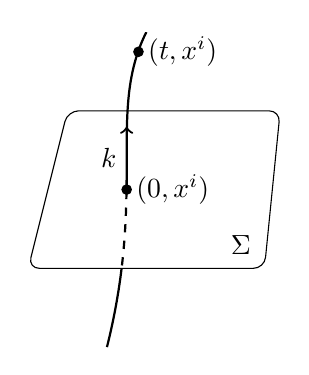
\begin{tikzpicture}
        \draw[rounded corners] (0,0) -- (0.5,2) -- (3.2,2) -- (3,0) -- cycle;
        \def\killingone{\draw[thick] (1,-1) .. controls (1.5,1) and (1,2) .. (1.5,3)}
        \begin{scope}
            \clip (0,0) rectangle (3,-1);
            \killingone;
        \end{scope}
        \begin{scope}[dashed]
            \clip (0,1) rectangle (3,0);
            \killingone;
        \end{scope}
        \begin{scope}
            \clip (0,1) rectangle (3,3);
            \killingone;
        \end{scope}
        \draw[fill] (1.25,1) circle (0.06) node[right] {\((0,x^i)\)};
        \draw[->,thick] (1.25,1) -- (1.25,1.8) node[midway,left] {\(k\)};
        \draw[fill] (1.4,2.75) circle (0.06) node[right] {\((t,x^i)\)};
        \node at (2.7,0.3) {\(\Sigma\)};
    \end{tikzpicture}
\end{wrapfigure}

Suppose we have a stationary spacetime with timelike Killing vector \(k\). Let \(\Sigma\) be a spacelike 3 dimensional hypersurface, and let \(x^i\), \(i=1,2,3\) be coordinates on \(\Sigma\).

We define coordinates for the manifold in the following way: from each point \((x^1,x^2,x^3)\) extend an integral curve of \(k\); the point \((t,x^i)\) is a parameter distance \(t\) along this curve.

In the chart \((t,x^i)\), we can write:
\begin{equation}
    k=\pdv{t}
\end{equation}
Then, using the defining property of Killing vectors, we have that the metric is independent of \(t\). Thus, we can write:
\begin{equation}
    \dd{s}^2 = g_{00}(x^k)\dd{t}^2 + 2g_{0i}(x^k)\dd{t}\dd{x^i} + g_{ij}(x^j)\dd{x^i}\dd{x^j}
\end{equation}
and we have \(g_{00}<0\) since \(k\) is timelike.

Suppose we have a surface \(\Sigma\) given by \(f(x)=0\), where \(f:\mathcal{M}\rightarrow\RR\), \(\dd{f}|_\Sigma\ne0\). Then \(\dd{f}\) is normal to \(\Sigma\). Suppose \(n\) is another 1-form that is normal to \(\Sigma\). Then we can write \(n=g\dd{f}+fn'\), where \(g\) is a function and \(n'\) is some 1-form. We have:
\begin{equation}
    \dd{n} = \dd{g}\wedge\dd{f}+g\underbrace{\dd[2]{f}}_{=0} + \dd{f}\wedge n' + f\dd{n'}
\end{equation}
\begin{equation}
    \implies \dd{n}|_\Sigma = (\dd{g}-n')\wedge\dd{f} \implies n\wedge \dd{n}|_\Sigma = 0
\end{equation}
In fact, the converse is true:
\begin{theorem}[Frobenius]
    If \(n\) is a 1-form such that \(n\wedge \dd{n}=0\), then there exist functions \(f,g\) such that \(n=g\dd{f}\), so that \(n\) is normal to surfaces of constant \(f\).
\end{theorem}
If \(n\) is a 1-form of this type, we say it is \emph{hypersurface-orthogonal}.

\begin{defn}
    \((\mathcal{M},g)\) is \emph{static} if it contains a hypersurface-orthogonal timelike KVF.
\end{defn}

Suppose we are in a static spacetime, and define coordinates \(t,x^i\) as before. \(\Sigma\) is a surface of constant \(t\), so we have \(k \propto dt\), \(k_\mu \propto (1,0,0,0)\). Also note that \(k_\mu = g_{\mu\nu}k^\nu = g_{\mu\nu}(\pdv{t})^\nu = (g_{00},g_{10},g_{20},g_{30})\). Hence we can deduce that \(g_{i0}=0\), and can write the metric as:
\begin{equation}
    \dd{s}^2 = g_{00}(x^k) \dd{t}^2 + g_{ij}(x^k)\dd{x^i}\dd{x^j}
\end{equation}
where as before \(g_{00}<0\). In this metric we have a discrete isometry \((t,x^i) \rightarrow (-t,x^i)\). A static metric must be time-independent \emph{and} invariant under time reversal. A simple case of a stationary but not static metric is that associated with a rotating star. If we reverse time the star spins in the other direction.

\subsection{Static, spherically symmetric spacetimes}
If we have a spacetime that is both stationary and spherically symmetric, then the isometry group must contain:
\begin{equation}
    \underbrace{\RR}_{\substack{\text{time}\\\text{translation}}} \times \underbrace{SO(3)}_{S^2 \text{ orbits}}
\end{equation}
It can be shown that with this condition the spacetime must also be static.

Let \(\Sigma_t \perp k^a\) be a foliation of the spacetime, and use coordinates \((r,\theta,\phi)\) on each surface, where \(\theta,\phi\) are the usual spherical coordinates and \(r\) is the area-radius function as defined earlier. Then we must have:
\begin{equation}
    \dd{s}^2|_{\Sigma_t} = e^{2\Psi(r)}\dd{r}^2 + r^2\dd{\Omega}
\end{equation}
for some function \(\Psi(r)\). Note that we have no \(\dd{r}\dd{\theta}\) or \(\dd{r}\dd{\phi}\) terms because they would violate spherical symmetry. If we define \(t\) as above we can then write the entire metric as:
\begin{equation}
    \dd{s}^2 = -e^{2\Phi(r)}\dd{t}^2 + e^{2\Psi(r)}\dd{r}^2 + r^2\dd{\Omega}
\end{equation}
for some other function \(\Phi(r)\).

\subsection{The TOV equations}
Consider now the matter inside a stationary and spherically symmetric star. We will model the star as a perfect fluid, which means we have the following energy-momentum tensor:
\begin{equation}
    T_{ab} = (\rho+P)u_au_b + \rho g_{ab}
\end{equation}
where \(\rho\) is the energy density, \(P\) is the pressure, and \(u_a\) is the 4-velocity of the fluid. Since the star is stationary, we can assume the fluid is at rest, so \(u^a = e^{-\Phi}\left( \pdv{t} \right)^a\) (since \(u\) is a unit vector pointing in the \(t\) direction). Also, since we have spherical symmetry we can assume that \(\rho\) and \(P\) are functions of \(r\) only.

\lecture{18/01/16}
Make the following definition:
\begin{equation}
    e^{2\Psi(r)} = \left( 1 - \frac{2m(r)}{r} \right)^{-1}
\end{equation}
Note that since \(e^{2\Psi(r)}>0\), we have \(m(r) < \frac{r}{2}\). Using the Einstein field equations \(G = 8\pi T\) it is now possible to derive the \emph{Tolman-Oppenheimer-Volkoff equations}:

\begin{equation}
    \dv{m}{r} = 4\pi r^2\rho
    \tag{TOV1}
    \label{TOV1}
\end{equation}
\begin{equation}
    \dv{\Phi}{r} = \frac{m+4\pi r^3P}{r(r-2m)}
    \tag{TOV2}
    \label{TOV2}
\end{equation}
\begin{equation}
    \dv{P}{r} = - (P+\rho) \frac{m+4\pi r^3P}{r(r-2m)}
    \tag{TOV3}
    \label{TOV3}
\end{equation}
We now have three equations, but four unknowns (\(m\),\(\Phi\),\(\rho\) and \(P\)). In order to solve this system, we will need a fourth equation, and the one most commonly chosen is an equation of state relating \(P\) and \(\rho\). In a cold star, we can assume that the temperature \(T(\rho,P)=0\) and we can solve this to get \(P\) explicitly in terms of \(\rho\):
\begin{equation}
    P = P(\rho)
\end{equation}
This is called a \emph{barotropic} equation of state.

We will assume that \(\rho,P>0\). We will also assume that \(\dv{P}{\rho}>0\); this is a stability condition\footnote{Consider \(\dv{P}{\rho}<0\). Then if \(\rho\) increases by a small amount in a region \(R\), \(P\) decreases in \(R\), but then this causes more fluid to flow into \(R\), increasing \(\rho\) further.}. 

Let the radius of the star be \(R\).
\begin{description}
    \item[Outside the star] (\(r>R\)) we can assume \(\rho = P = 0\). \eqref{TOV1} then gives that \(m(r) = M\) a constant. \eqref{TOV2} further provides that \(\Phi = \frac{1}{2}\log\left( 1-\frac{2M}{r} \right) + \Phi_0\), where \(\Phi_0\) is another constant. Note that since \(g_tt = -e^{2\Phi} \rightarrow e^{-2\Phi_0}\) as \(r\rightarrow\infty\), we can eliminate \(\Phi_0\) by making a change of coordinates \(t\rightarrow e^{\Phi_0}t\), so w.l.o.g. we assume that \(\Phi_0 = 0\).
        Hence we have the \emph{Schwarzschild metric}:
        \begin{equation}
            \dd{s}^2 = - \left( 1 - \frac{2M}{r} \right)\dd{t}^2 + \left( 1 - \frac{2M}{r} \right)^{-1}\dd{r}^2 + r^2\dd{\Omega}^2
        \end{equation}
        By taking \(r\) to be large and comparing with Newtonian gravity, we can deduce that \(M\) is in fact the mass of the star.
        Note that this metric has a problem. It is singular at the so-called \emph{Schwarzschild radius} \(r=2M\). Thus a static, spherically symmetric star must have \(R>2M\) (in a normal star, \(R\gg2M\)).
    \item[Inside the star] (\(r<R\)), we now have matter to deal with. Integrating \eqref{TOV1}, we have:
        \begin{equation}
            m(r) = 4\pi\int_0^r\rho(r')r'^2\dd{r'}+m_*
        \end{equation}
        where \(m_*\) is a constant. Consider a constant \(t\) hypersurface. The induced line element on this hypersurface is \(\dd{s}^2 = e^{2\Psi}\dd{r}^2 + r^2\dd{\Omega}^2\). The proper radius (i.e. distance to \(r=0\)) of a point is given by \(\int_0^re^{\Psi(r')}\dd{r'}\). In order for our spacetime to be a manifold, we require that it is locally flat at \(r = 0\), and this requires that the proper radius tends to the area-radius as \(r\rightarrow 0\). Note that
        \(\int_0^re^{\Psi(r')}\dd{r'} \sim e^{\Psi(0)}r\) as \(r\rightarrow 0\), so we require that \(e^{\Psi(0)} = 1\), or equivalently \(m(0) = 0\). From this we deduce that \(m_*=0\). 

        If we match this expression on the boundary of the star to the Schwarzschild solution for the exterior, we see that \(m(R)=M\), or:
        \begin{equation}
            M = 4\pi\int_0^R\rho(r)r^2\dd{r}
            \tag{\(*\)}
            \label{match}
        \end{equation}
        The volume form on a constant \(t\) hypersurface is \(e^\Psi r^2\sin\theta \dd{r}\wedge\dd{\theta}\wedge\dd{\phi}\), and so the energy of the matter in the star for \(t\) constant is:
        \begin{equation}
            E = 4\pi\int_0^R\rho e^\Psi r^2\dd{r}
        \end{equation}
        Note that since \(m\) is increasing, so is \(e^\Psi\) and hence \(e^\Psi\ge1\) for all \(0 \le r \le R\). Thus we have \(E > M\). The reason for this is that we have a gravitational binding energy \(E-M\).

        If we evaluate \(\frac{m(r)}{r}<\frac{1}{2}\) at \(r=R\) we see that \(\frac{M}{R} < \frac{1}{2}\). In fact it is possible to improve this: \eqref{TOV3} \(\implies\dv{P}{r}\le0\implies\dv{\rho}{r}\le0\), and from this we can deduce:
        \begin{equation}
            \frac{m(r)}{r} < \frac{2}{9}\left( 1 - 6\pi r^2P(r) + \left[ 1 + 6\pi r^2P(r) \right]^{\frac{1}{2}} \right)
            \tag{\(\dagger\)}
            \label{buchdahl}
        \end{equation}
        Setting \(r = R\) and noting \(P(R) = 0\), we obtain the so-called \emph{Buchdahl inequality}: \(\frac{M}{R}<\frac{4}{9}\).

        In general, we must solve this system of equations numerically. \eqref{TOV1} and \eqref{TOV3} are a pair of coupled first order ODEs for \(m(r)\) and \(\rho(r)\), from which we can obtain a unique solution given \(m(0)=0\) and specifying \(\rho(0) = \rho_c\), the central density. From \eqref{TOV3} we have that \(P\) is decreasing in \(r\), so \(R(\rho_c)\) is determined by fixing \(P(R) = 0\). Then, using \eqref{match} we can obtain \(M(\rho_c)\). Finally, using
        \eqref{TOV2} and the boundary condition that \(\Phi(R) = \frac{1}{2}\log\left( 1 - \frac{2M}{R} \right)\) we can deduce \(\Phi(r)\). 

        To summarise, given an equation of state, static, spherically symmetric, cold stars are a 1-parameter family labelled by \(\rho_c\).
\end{description}

\subsection{Maximum mass}
We wish to find a limit on the maximum mass of a star.
\begin{figure}[H]
    \centering
    \begin{tikzpicture}[scale=1.5]
        \draw[domain=0:3,smooth,variable=\x] plot({\x},{\x*(3.2-\x)/2});
        \draw[thick,->] (0,0) -- (3.5,0) node[right] {\(\rho_c\)};
        \draw[thick,->] (0,0) -- (0,1.6) node[above] {\(M\)};
        \draw[dashed] (0,1.28) node[left] {\(M_{\text{max}}\)} -- (3.5,1.28);
    \end{tikzpicture}
\end{figure}
In general, \(M_{\text{max}}\) depends on the equation of state, but here we run into a problem: we do not know the equation of state in certain conditions, namely \(\rho>\rho_0\), where \(\rho_0\) is typically on the order of the density of an atomic nucleus.

\begin{wrapfigure}{l}{0.5\linewidth}
    \centering
    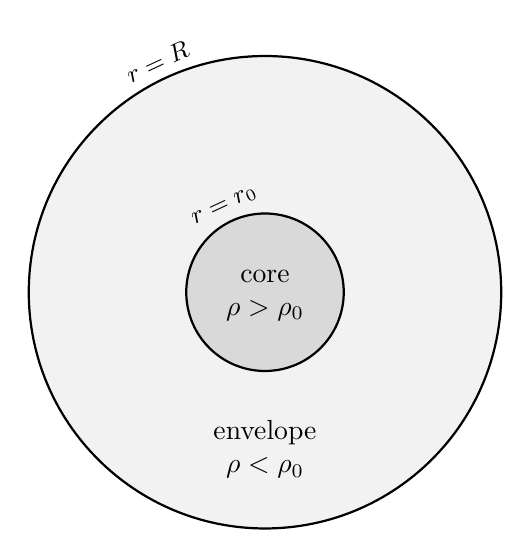
\begin{tikzpicture}
        \fill[gray!10] (0,0) circle (3);
        \fill[gray!30] (0,0) circle (1);
        \draw[thick] (0,0) circle (3);
        \draw[thick] (0,0) circle (1);

        \node at (0,0) {
            \begin{tabular}{c}
                core \\
                \(\rho>\rho_0\)
            \end{tabular}
            };
        \node at (0,-2) {
            \begin{tabular}{c}
                envelope \\
                \(\rho<\rho_0\)
            \end{tabular}
            };
        
        \node[above,rotate=25,shift={(0,1)}] at (0,0) {\small\(r=r_0\)};
        \node[above,rotate=25,shift={(0,3)}] at (0,0) {\small\(r=R\)};
    \end{tikzpicture}
\end{wrapfigure}
Remarkarbly, it is still possible to find an upper bound on the mass of a star. We do this by splitting the star into two regions: an \emph{envelope}, in which we know the equation of state (so \(\rho<\rho_0\)), and a \emph{core}, in which we do not (\(\rho>\rho_0\)). Since \(\dv{\rho}{r}<0\), the envelope does in fact envelope the core.

Let \(m_0 = m(r_0)\); we call this the \emph{core mass}. Since the minimum density in the core is \(\rho_0\), we have \(m_0\ge\frac{4}{3}\pi r_0^3\rho_0\). Additionally, we can apply \eqref{buchdahl} at \(r=r_0\) to obtain:
\begin{equation}
    \frac{m_0}{r_0} < \frac{2}{9}\left( 1 - 6\pi r_0^2P_0 + \left[ 1 + 6\pi r_0^2P_0 \right]^{\frac{1}{2}} \right)
\end{equation}
where \(P_0=P(\rho_0)\). This is a decreasing function of \(P_0\), so \(\frac{m_0}{r_0}<\frac{4}{9}\).

Lets plot these two constraints:
\begin{figure}[H]
    \centering
    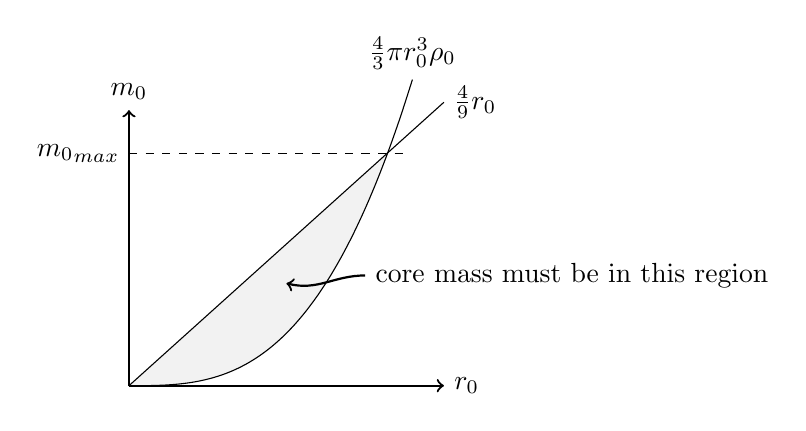
\begin{tikzpicture}
        \begin{scope}
            \clip (0,0) -- (4,0) -- (4,3.6) -- cycle;
            \fill[gray!10,domain=0:3.6,smooth,variable=\x] plot({\x},{\x^3/12});
        \end{scope}<++>
        \draw[domain=0:3.6,smooth,variable=\x] plot({\x},{\x^3/12}) node[above] {\(\frac{4}{3}\pi r_0^3\rho_0\)};
        \draw[domain=0:4,smooth,variable=\x] plot({\x},{\x*0.9}) node[right] {\(\frac{4}{9}r_0\)};
        \draw[thick,->] (0,0) -- (4,0) node[right] {\(r_0\)};
        \draw[thick,->] (0,0) -- (0,3.5) node[above] {\(m_0\)};
        \draw[dashed] (0,2.95) node[left] {\({m_0}_{\text{max}}\)} -- (3.5,2.95);

        \draw[thick,<-] (2,1.3) .. controls (2.4,1.2) and (2.6,1.4) .. (3,1.4) node[right] {core mass must be in this region};
    \end{tikzpicture}
\end{figure}
We see that we have an upper bound on the core mass. Solving for this upper bound, we find:
\begin{equation}
    m_0 < \sqrt{\frac{16}{23\pi\rho_0}}
\end{equation}
If \(\rho_0\approx\) nuclear density, then we have \(m_0 \lesssim 5M_{\astrosun}\).

Now we can extend our solution to the envelope. \(m_0\) and \(r_0\) together uniquely determine the envelope, as we can solve \eqref{TOV1} and \eqref{TOV3} starting at \(r=r_0\) and using the known equation of state for \(\rho<\rho_0\). From this we obtain \(M\) as a function of \(m_0\) and \(r_0\), and so can find the maximal value of \(M\) when \(m_0,r_0\) take values in the region in the graph above.

Numerically, we can find that \(M\) is maximised when \(m_0\) is maximised, and that the maximum mass is \(M\approx m_0\approx5M_{\astrosun}\).

In fact, it is possible to improve this limit by imposing that the speed of sound is physical, i.e. less than the speed of light: \(\sqrt{\dv{P}{\rho}}\le1\). Using this gives \(M \lesssim 3M_{\astrosun}\).

\end{document}
